\documentclass{beamer}
\usetheme{boxes}

\setbeamertemplate{navigation symbols}{}
\setbeamertemplate{itemize item}{\color{azure}$\blacksquare$}
\setbeamercolor{frametitle}{fg=azure}
\setbeamercolor{title}{fg=azure}
\setbeamercolor{framesubtitle}{fg=azure}
\setbeamercolor{block title}{fg=azure}



\usepackage{fontspec}
\setmainfont{Raleway}

\AtBeginSection[]{
  \begin{frame}
  \vfill
  \centering
  \begin{beamercolorbox}[sep=8pt,center,shadow=true,rounded=true]{title}
    \usebeamerfont{title}\insertsectionhead\par%
  \end{beamercolorbox}
  \vfill
  \end{frame}
}

\usepackage{emoji}

\usepackage{xcolor}
\definecolor{azure}{rgb}{0.0, 0.5, 1.0}
\definecolor{awesome}{rgb}{1.0, 0.13, 0.32}

\usepackage{svg}

\usepackage[
    type={CC},
    modifier={by-nc-sa},
    version={3.0},
]{doclicense}

\title[JOSS]{The Journal of Open Source Software: Developing a Software Review Community} % The short title appears at the bottom of every slide, the full title is only on the title page

\author{Patrick Diehl} 
\institute[LSU] % Your institution as it will appear on the bottom of every slide, may be shorthand to save space
{
Applied Computer Science \\ Los Alamos National Laboratory \\ Department of Physics and Astronomy \\ Louisiana State University \\ % Your institution for the title page
\medskip
\textit{diehlpk@lanl.gov} % Your email address
}


\begin{document}

\begin{frame}
\titlepage
\end{frame}

\begin{frame}{Motivation}

\begin{center}
    \textcolor{azure}{(Open source) software is essential for computational sciences}
\end{center}

\textbf{For example}, developing an R, C\texttt{++}, or Python package with some novel algorithms which are widely used by the research community is cool, but might not yet be considered for promotions, grant applications, or for awarding tenure. \emoji{astonished}\\
\vspace{0.25cm}
\textbf{Funding}: NSF's Pathways to Enable Open-Source Ecosystems (POSE)\footnote{\tiny\url{https://new.nsf.gov/funding/opportunities/pose-pathways-enable-open-source-ecosystems}}. \emoji{clap}\\
\vspace{0.25cm}
\textcolor{awesome}{Contrary}, people get credit for papers (citations) using open source software. How can we change that, and people get credit for software? \emoji{thinking} 
\end{frame}

\begin{frame}
\frametitle{Overview} % Table of contents slide, comment this block out to remove it
\tableofcontents % Throughout your presentation, if you choose to use \section{} and \subsection{} commands, these will automatically be printed on this slide as an overview of your presentation
\end{frame}

%------------------------------------------------
%\section{The Journal of Open Source Software: Developing a Software Review Community} % Sections can be created in order to organize your presentation into discrete blocks, all sections and subsections are automatically printed in the table of contents as an overview of the talk
%------------------------------------------------

%\subsection{Subsection Example} % A subsection can be created just before a set of slides with a common theme to further break down your presentation into chunks

\begin{frame}{Journal of Open Source Software}
\begin{center}

\includegraphics{joss.png}    
\end{center}

{\fontsize{4}{8}\selectfont
\textbf{Patrick Diehl}, Daniel S.~Katz, Gabriela Alessio Robles, Stefan Appelhoff, Warrick Ball,  Mojtaba Barzegari, Johanna Bayer,  Juanjo Bazán,  Sophie Beck,  Sebastian Benthall, Eloisa Bentivegna,  Monica Bobra,  Frederick Boehm, Sébastien Boisgérault, Josh Borrow, Teon Brooks, Jed Brown, Philip Cardiff, Taher Chegini,  Beatriz Costa Gomes, Pierre de Buyl, Renata Diaz,  Axel Donath, Elizabeth DuPre, Matthew Feickert, Vissarion Fisikopoulos, Martin Fleischmann, Samuel Forbes, Dan Foreman-Mackey, Jarvist Moore Frost, Nikoleta Glynatsi, Jeff Gostick, Rohit Goswami, Richard Gowers, Hugo Gruson, Olivia Guest, Jayaram Hariharan, Gracielle Higino, Susan Holmes, Luiz Irber, Adam R. Jensen, Mark A. Jensen, Prashant K Jha, Sehrish Kanwal, Vincent Knight, Olexandr Konovalov, Rachel Kurchin, Paul La Plante, Oskar Laverny, Hugo Ledoux, Christopher R. Madan, Michael Mahoney, Brian McFee, Rocco Meli, Sarath Menon, Antonia Mey, Tristan Miller, Kevin M. Moerman, Ivelina Momcheva, Yasmin Mzayek, Kanishka B. Narayan, Kyle Niemeyer, Lorena Pantano, Andrew Quinn, AHM Mahfuzur Rahman, Julia Romanowska, Kelly Rowland, Anjali Sandip, Mehmet Hakan Satman, Jonny Saunders, Fabian Scheipl, Jacob Schreiber, Hauke Schulz, Adi Singh, Arfon Smith, Dana Solav, Claudia Solis-Lemus, Charlotte Soneson, Øystein Sørensen, Andrew Stewart, Marcel Stimberg, Fabian-Robert Stöter, Fei Tao, George K. Thiruvathukal, Kristen Thyng, Ana Trisovic, Adam Tyson, Chris Vernon, Marcos Vital, Rachel Wegener, Britta Westner, Lucy Whalley, Frauke Wiese, Mengqi Zhao, and Bonan Zhu.}

\begin{center}
     \url{https://joss.theoj.org}
\end{center}

\end{frame}

\section{How to better recognize software
contributions?}

\begin{frame}{How to better recognize software
contributions?}

\begin{itemize}
    \item Find some way to fit software into
current (paper/book-centric)
system
    \item  Evolve beyond one-dimensional
credit model
\end{itemize}

\begin{center}
    \textcolor{blue}{What if we just wrote papers about software?}
\end{center}

\begin{itemize}
    \item<only@1> Gives us something easy to cite \emoji{thumbs-up-light-skin-tone}
    \item<only@1> No changes required to existing
infrastructure \emoji{ok-hand-medium-dark-skin-tone}
    \item<only@1> Publishing in existing journals raises
profile of software within a community \emoji{love-you-gesture-medium-skin-tone}
%
    \item<2> Writing another paper can be a ton of
work \emoji{grinning-face-with-sweat}
    \item<2> Many journals don’t accept software
papers \emoji{face-with-symbols-on-mouth}
    \item<2> For long-lived software packages, static
authorship presents major issues \emoji{worried-face}
    \item<2> Many papers about the same software
may lead to citation dilution \emoji{oncoming-fist-light-skin-tone}
\end{itemize}

    
\end{frame}

\begin{frame}

\begin{center}
What if we made it as easy as
possible to write and publish a
software paper?
\end{center}

\begin{center}
   \textcolor{blue}{Embracing the hack}
\end{center}

\end{frame}

\section{Submission process}

\begin{frame}
  
\includegraphics[scale=0.5]{joss.png}      \includesvg{joss-text.svg}
\vspace{1cm}
\begin{itemize}
    \item A \textbf{developer-friendly} journal* for research software
packages
    \item Paper preparation (and submission) for well-documented
software should take \textbf{no more than an hour}
\item The primary purpose of a JOSS paper is to \textbf{enable citation
credit} to be given to authors of research software
\end{itemize}

\vspace{2cm}

{tiny * Other (commercial) venues exist for publishing papers about software}
\end{frame}

    
\begin{frame}{JOSS process {\tiny(\url{https://doi.org/10.6084/m9.figshare.5147773.v2})}}
    \centering
    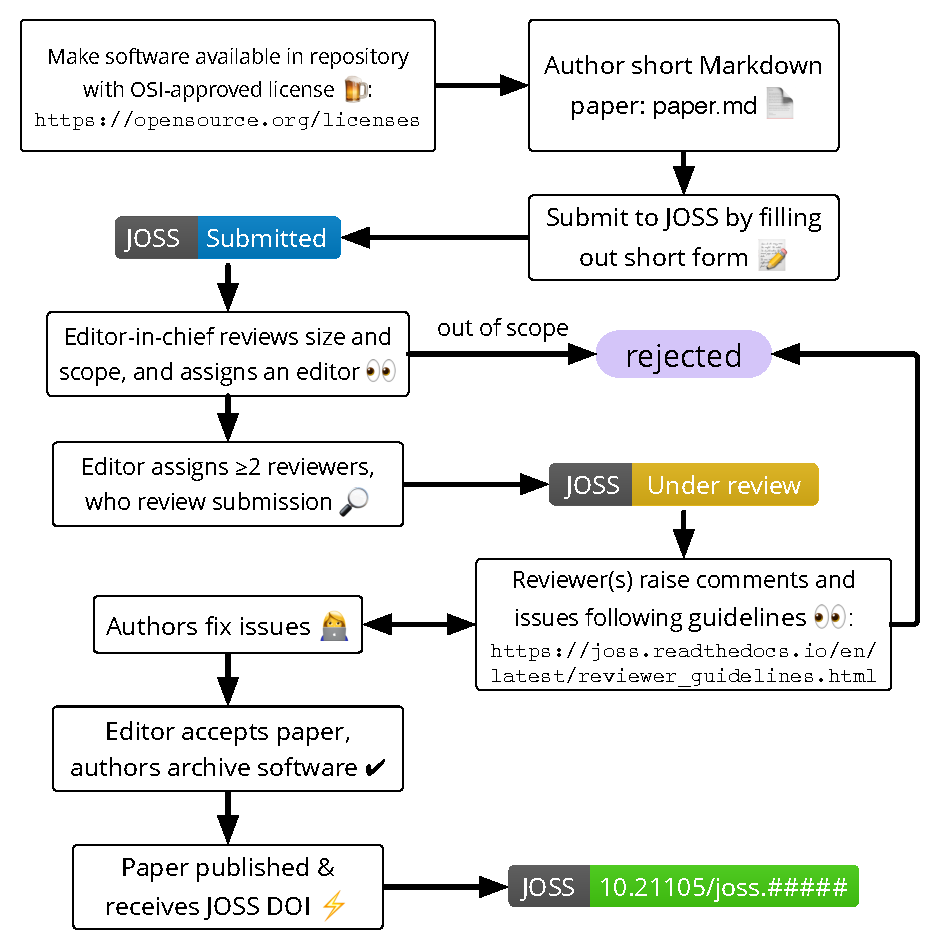
\includegraphics[scale=0.5]{JOSS-flowchart-updated.pdf}
\end{frame}

\begin{frame}{JOSS - Review Checklist}

\begin{itemize}
    \item Agree to Conflict of Interest \& Code of Conduct
    \item General checks: repository URL, license,
contribution and authorship
    \item Functionality: installation, functional claims,
performance
\item Documentation: statement of need, installation
instructions, example usage, functionality
documentation, automated tests, community
guidelines
\item Software paper: summary, statement of need,
state of the field, quality of writing, references
\end{itemize}
    
\end{frame}


\begin{frame}{JOSS - Review Checklist Details}
Definition of each check-in JOSS documentation:
\url{https://joss.readthedocs.io/en/latest/
review_criteria.html}\\
\vspace{0.5cm}
The editor helps the reviewer and author come to
agreement and some criteria have guidance
\vspace{0.5cm}
\begin{itemize}
    \item Installation
    \item API documentation
    \item Community guidelines
    \item Automated testing
\end{itemize}
    
\end{frame}

\begin{frame}{JOSS - Review Checklist Details}
\framesubtitle{Installation}

\begin{itemize}
    \item \emoji{thumbs-up-medium-skin-tone}: The software is simple to install, and
follows established distribution and dependency
management approaches for the language
being used
\item \emoji{oncoming-fist-dark-skin-tone}: A list of dependencies to install, together
with some kind of script to handle their
installation (\emph{e.g.}, a Makefile)
\item \emoji{thumbs-down-light-skin-tone} (not acceptable): Dependencies are unclear,
and/or installation process lacks automation
\end{itemize}
    
\end{frame}

\begin{frame}{JOSS - Review Checklist Details}
\framesubtitle{API Documentation}

\begin{itemize}
        \item \emoji{thumbs-up-medium-skin-tone}: All functions/methods are documented
including example inputs and outputs
\item \emoji{oncoming-fist-dark-skin-tone}: Core API functionality is documented
\item \emoji{thumbs-down-light-skin-tone} (not acceptable): API is undocumented
\end{itemize}
    
\end{frame}

\begin{frame}{JOSS - Review Checklist Details}
\framesubtitle{Automated Tests}

\begin{itemize}
        \item \emoji{thumbs-up-medium-skin-tone}: An automated test suite hooked up to
continuous integration (GitHub Actions, Circle CI,
or similar)
\item \emoji{oncoming-fist-dark-skin-tone}: Documented manual steps that can be
followed to objectively check the expected
functionality of the software (\emph{e.g.}, a sample input
file to assert behavior)
\item \emoji{thumbs-down-light-skin-tone} (not acceptable):  No way for you, the
reviewer, to objectively assess whether the
software works
\end{itemize}
    
\end{frame}

\begin{frame}{JOSS as a Community}
    \begin{itemize}
        \item Cultures change based on rules and incentives
        \item JOSS practices have influenced reviewers and
developers in terms of what's good and what's
minimally acceptable
\item Similar to rOpenSci's influence in the R community
\item JOSS provides rules, and at a high-level, tries to
nudge incentives
\item Accepted software = accepted paper
\item If software was cited directly, JOSS papers wouldn't
be needed, but JOSS reviews and JOSS
community would still have great value
    \end{itemize}
\end{frame}

\section{Editorial bot}

\begin{frame}\frametitle{Bot-based process using GitHub: @editorialbot}

    \begin{columns}
    \column{0.5\textwidth}
    \begin{itemize}
        \item Interacts with authors, reviewers, and editors
in review ‘issues’ on GitHub
\item Compiles papers (Pandoc)
\item Conducts automated ‘healthchecks’ for
incoming submissions (\emph{e.g.}\ license checks,
search for missing DOIs)
\item Sends automated reminders
\item Deposits metadata and
 and 
registers DOIs with Crossref
    \end{itemize}
        
    \column{0.6\textwidth}
        \centering
        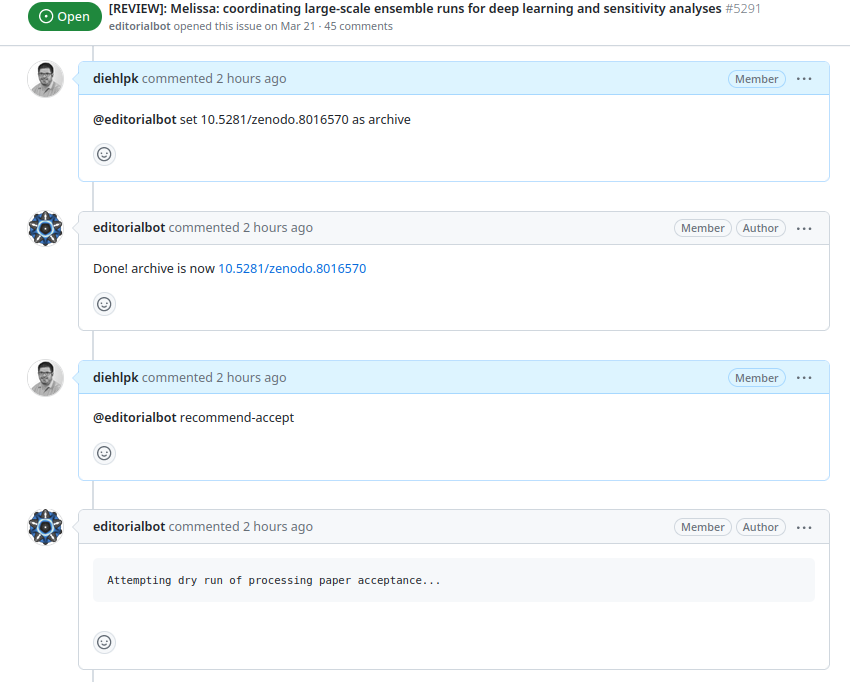
\includegraphics[width=\textwidth]{joss-github.png}
    \end{columns}

\end{frame}

\section{10 years of JOSS in numbers}

\begin{frame}{Some data on most cited papers}

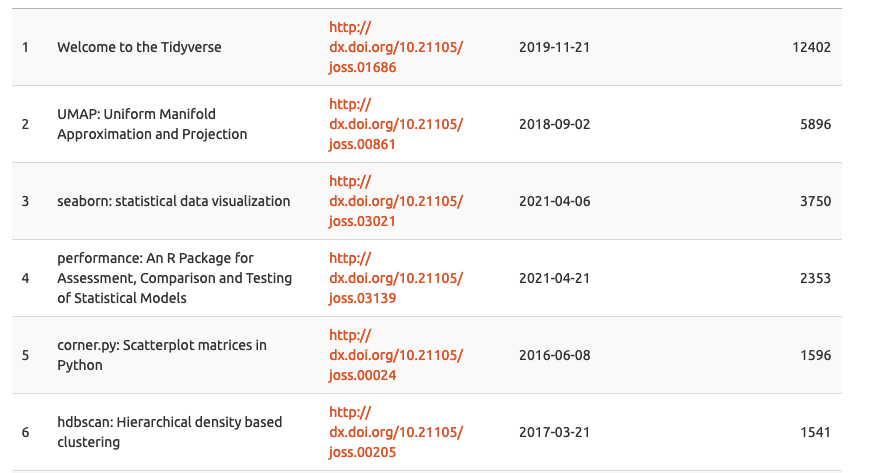
\includegraphics[width=\linewidth]{most-cited.png}



{\tiny More data: \url{http://www.theoj.org/joss-analytics/joss-submission-analytics.html}}    
\end{frame}

\begin{frame}{Some data on published papers}

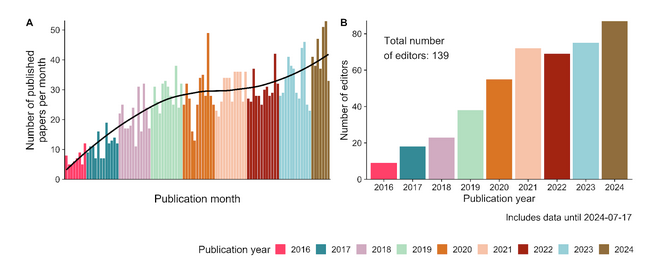
\includegraphics[width=\linewidth]{papers-per-year.png}



{\tiny More data: \url{http://www.theoj.org/joss-analytics/joss-submission-analytics.html}}    
\end{frame}


\section{Costs per JOSS paper? Disclaimer: JOSS has no publication fee!}

\begin{frame}{ \emoji{heavy-dollar-sign} How much does it cost to publish one paper?}
\framesubtitle{JOSS has no publication or open access fees! \emoji{clapping-hands}}

\begin{block}{Costs in 2019\footnote{\tiny\url{https://blog.joss.theoj.org/2019/06/cost-models-for-running-an-online-open-journal}}}
\begin{itemize}
\item  Annual Crossref membership: \$275/year
\item  JOSS paper DOIs: \$1/accepted paper
\item  JOSS website hosting: \$19/month
\item  JOSS domain name registration: \$10/year
\end{itemize}
\end{block}
At 300 papers/year in 2019, this is \$813, or \$2.71/paper. This is what we actually pay today, covered by a grant from the Alfred P. Sloan Foundation.\\
\vspace{0.5cm}
Today, a more accurate cost is probably around \$4-US\$5 per paper, though this hasn't been formally calculated, including services such as web hosting, Crossref membership and services, Portico preservation services, etc. 

\end{frame}

\begin{frame}{No publication fees? Who finances JOSS? \emoji{detective}}

\begin{itemize}
\item \$50 for each paper that comes from AAS (24 such papers have been published by JOSS)
\item \$20k gift from the Gordon and Betty Moore Foundation to start up the journal infrastructure 
\item \$380k grant from Alfred P. Sloan Foundation to improve the infrastructure and generalize it to be useful to other parts of the scholarly publishing community. 
\item Some authors donated to JOSS after the paper was accepted.
\end{itemize}

\end{frame}



%\section{Floss for Science: A podcast promoting open source software}

\begin{frame}{Floss for Science}
\framesubtitle{A podcast promoting open source software}

    \begin{columns}
    \column{0.5\textwidth}
    \begin{itemize}
        \item \textit{FLOSS for Science} is a podcast with the goal of showcasing free, libre and open source software uses in science. 
        \item We want to highlight how FLOSS empowers researchers and enables them to produce high quality research. 
        \item So far 32 episodes published, however, we did a break during the pandemic
    \end{itemize}
        
    \column{0.6\textwidth}
        \centering
        
\includegraphics[width=0.75\textwidth]{floss-logo.png}
    \end{columns}
    \vspace{0.5cm}
Credits to David Brassard my co-host, who started the podcast with me in January 2018.
\end{frame}

\begin{frame}{Some selected episodes}
    \begin{minipage}{1\textwidth}
    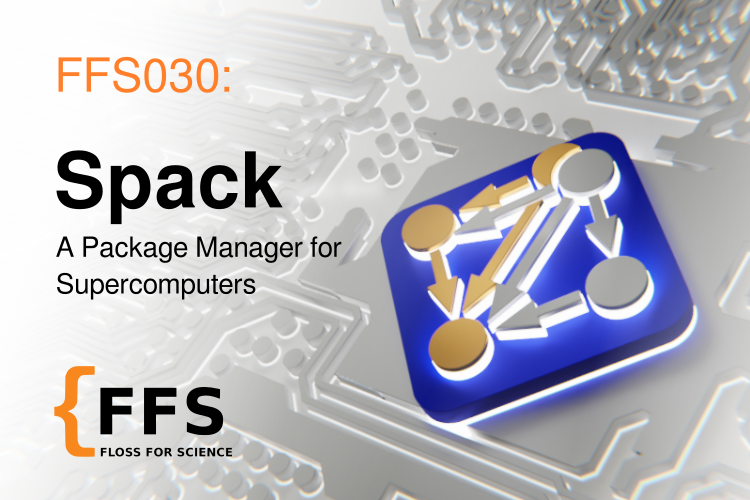
\includegraphics[width=0.5\linewidth]{FFS030_header.png}
    \hfill
    
\includegraphics[width=0.5\linewidth]{FFS028_header.png}\\
    \vspace{0.5cm}
    
\includegraphics[width=0.5\linewidth]{FFS027_header.png}
    \hfill
    
\includegraphics[width=0.5\linewidth]{FFS019_header.png}
  \end{minipage}
\end{frame}

\begin{frame}{Open source software for production}

    \begin{itemize}
        \item Low-cost hardware is readily available
        \item The software components required for high quality audio production are available with open source licenses under Linux
        \item It is strongly recommended to record every participant on individual audio tracks to adjust their audio level separately
        \begin{itemize}
            \item The setup to record a podcast with all participants on a single track will be significantly easier to prepare and manage, but we chose to go with a multitrack setup for high audio quality
        \end{itemize}
    \end{itemize}
    
\end{frame}

\begin{frame}{Open source software for production}

    Hardware setup for local and remote podcast recording (\textasciitilde \$400 -- \$450):
    \begin{itemize}
        \item Behringer UMC404HD audio interface (\$180)
        \begin{itemize}
            \item Up to 4 local participants
            \item One Shure SM58 (\$99) for each local participant
        \end{itemize}
        \item Samson Q2U USB microphone for remote participants (\$70)
        \begin{itemize}
            \item It is possible to avoid the purchase of an audio interface if all participants are remote
        \end{itemize}
        \item Other class-compliant audio interfaces and microphones are available
        \item One computer serves as a central node for the remote and local recording
        \begin{itemize}
            \item General use computers are plenty sufficient
            \item Recording for FFS was performed on either a Thinkpad W530 or a Thinkpad X260
            \item The computer will need stable network connectivity
        \end{itemize}
        \item A multichannel headphone amplifier (\$35) is strongly suggested to give audio feedback for all local participants and improve their posture while recording
    \end{itemize}

\end{frame}

\begin{frame}{Open source software for production}

    General software
    \begin{itemize}
        \item Jitsi.meet
        \begin{itemize}
            \item VOIP software for remote participants
            \item The only requirement for the participants is a WebRTC compatible web browser
        \end{itemize}
        \item Chromium
        \begin{itemize}
            \item Separate Jitsi.meet instances on different tabs
            \item Firefox did not allow splitting the audio from different tabs into multiple channels \emoji{worried-face}
        \end{itemize}
        \item Linux
        \begin{itemize}
            \item All packages are available in Ubuntu from the main or third-party repositories
            \item Any Linux distribution can be made to work
            \item Ubuntu Studio is an easy all-in-one solution for beginners
            \item Real time or low latency kernel are suggested but not absolutely required for less demanding recording situations such as podcast recording
        \end{itemize}
    \end{itemize}

\end{frame}

\begin{frame}{Open source software for production}

    Audio software
    \begin{itemize}
        \item JACK (will eventualy be replaced by PipeWire for an easier setup)
        \begin{itemize}
            \item JACK Audio Connection Kit
            \item Linux low latency audio stack
            \item Allow special routing between different sources and sinks
            \item Need to be properly configured to create bridges to PulseAudio
        \end{itemize}
    \end{itemize}

\begin{columns}

    \begin{column}{0.4\linewidth}
        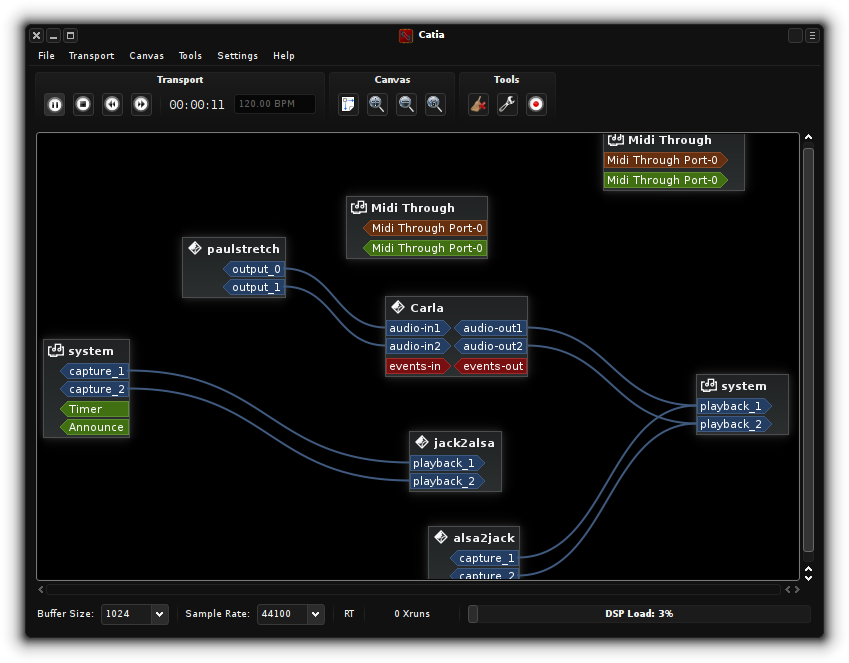
\includegraphics[width=\linewidth]{catia.png}
    \end{column}

    \begin{column}{0.6\linewidth}
        \begin{itemize}
            \item A JACK session manager and routing software (for graphical routing)
            \begin{itemize}
                \item Multiple combination/alternatives
                \item Cadence
                \item Ubuntu Studio Controls
                \item Qjackctl
                \item Catia
                \item Patchage
            \end{itemize}
        \end{itemize}
    \end{column}
    
    \end{columns}

\end{frame}

\begin{frame}{Open source software for production}

    Audio software

    \begin{columns}

    \begin{column}{0.4\linewidth}
        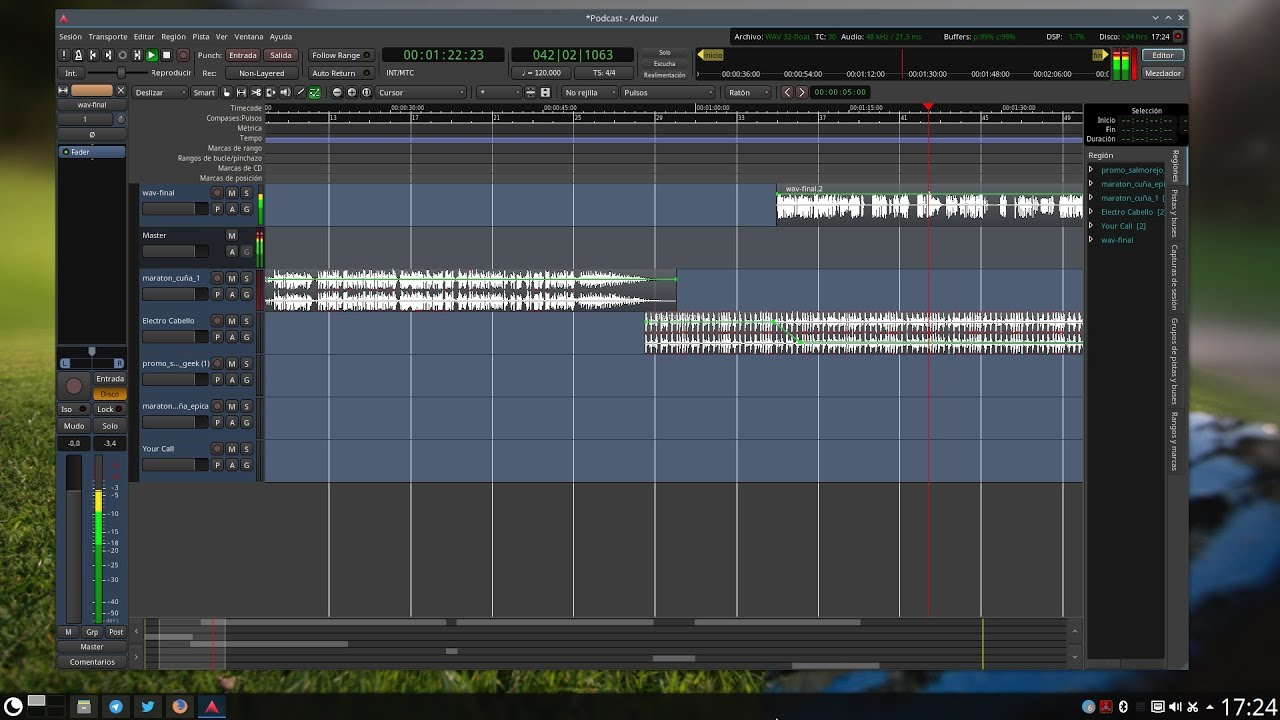
\includegraphics[width=\linewidth]{maxresdefault.jpg}
    \end{column}

    \begin{column}{0.6\linewidth}
        \begin{itemize}
            \item Ardour
            \begin{itemize}
                \item Multitrack audio recorder and editor
                \item Plugin host (denoise, gate, compressor, limiter, etc.)
            \end{itemize}
      
            \item CALF plugins
            \begin{itemize}
                \item Decent and easy to use audio plugins
                \item Gate, Compressor, Limiter...
            \end{itemize}
        \end{itemize}
    \end{column}
    
    \end{columns}

\vspace{6pt}

Other software and services
\begin{itemize}
    \item Media file hosting on Archive.org
    \item Website hosting on Github-pages
    \item Jeckyl static generated website
    \item Audio levelling with Auphonic online (non-free software)
\end{itemize}

\end{frame}


\begin{frame}{Lessons learned}

\begin{block}{Surprising}
    \begin{itemize}
        \item Was quite easy to find people willing to be interviewed,
        \item A professional graphic designer volunteered helping with the artwork
        \item Some episodes had over 600 listeners
    \end{itemize}
\end{block}

\begin{block}{Challenges}
    \begin{itemize}
        \item Was sometimes difficult to schedule interviews, \emph{e.g.}\ time zones, working hours.
        \item High quality audio is important, however, editing took much time out of David's resources.
        \item Funding is needed for editing, however, we want to avoid advertisement or sponsoring
    \end{itemize}
\end{block}
    
\end{frame}

\begin{frame}{Conclusion}

\begin{block}{Benefits \emoji{smiley}}
    \begin{itemize}
        \item JOSS is one opportunity to get credit for software development
        \item JOSS is a collaboration between author, editor and reviewers
    \end{itemize}
\end{block}

\begin{block}{Challenges \emoji{neutral-face}}
        \begin{itemize}
            \item  JOSS is funded by NumFocus, \emph{e.g.}\ server, DOI. However, all editors and reviewers are volunteers.
            \item Scalability! Last year 400 published papers means at least 800 reviewers. Do not burn our volunteers.
        \end{itemize}
\end{block}

 \emoji{pray} Please submit your software package and get credit for your work!\\
 \emoji{pray} Please sign up as reviewer to help JOSS to handle around 400 papers per year.


\tiny \doclicenseThis
\end{frame}

\end{document}


